\begin{figure*}
	\centering
	\vspace{0.5cm}
	\includegraphics{figures/fancy-figure.pdf}
 \caption{ This visualisation shows two epochs at once, simultaneously
 showing the initial conditions (in blue and red) and the final simulation
 volume at redshift $z=0$ in white/grey. The blue and red show the positions
 of the gas and dark matter (respectively) \emph{in the initial conditions}
 for particles that reside in selected haloes at redshift $z=0$. The overlaid
 white/grey map shows the dark matter at redshift $z=0$ to enable comparisons
 between the initial and final comoving positions for various bound
 structures. For each selected halo, the dashed black circles show their
 virial radii as defined in \S \ref{sec:simba}. For some haloes in crowded
 regions, we have overlaid a circle and arrows showing which blob of dark
 matter and gas in the initial conditions collapses to form this halo.
 Finally, for each halo we show a small bar chart showing how their gas is
 composed from Lagrangian components, as described later in the text. The
 blue bar shows the fraction of gas in each halo that originated from that
 haloes own Lagrangian region, the red bar shows the gas from another haloes
 Lagrangian region, and the purple bar shows the fraction of gas that
 originated outside any Lagrangian region. This figure illustrates the
 significant differences in origin between the gas (blue) and dark matter
 (red) for these selected haloes of various masses. We also see how the
 environment of each halo changes its Lagrangian make-up. In particular,
 group 431 shows a large baryonic component originating from the Lagrangian
 region of another halo, with this halo entering a small cluster environment
 near the end of the simulation. Note that individual regions are
 colour-mapped separately, i.e. the intensity of colour for a single halo is
 unique to that halo only, as to enable all Lagrangian regions to be seen.
 Without this choice, the structure for the lower mass haloes would be
 completely washed out.}
	\vspace{1cm}
	\label{fig:bigtransferpic}
\end{figure*}


\begin{figure*}
    \centering
    \vspace{1cm}
    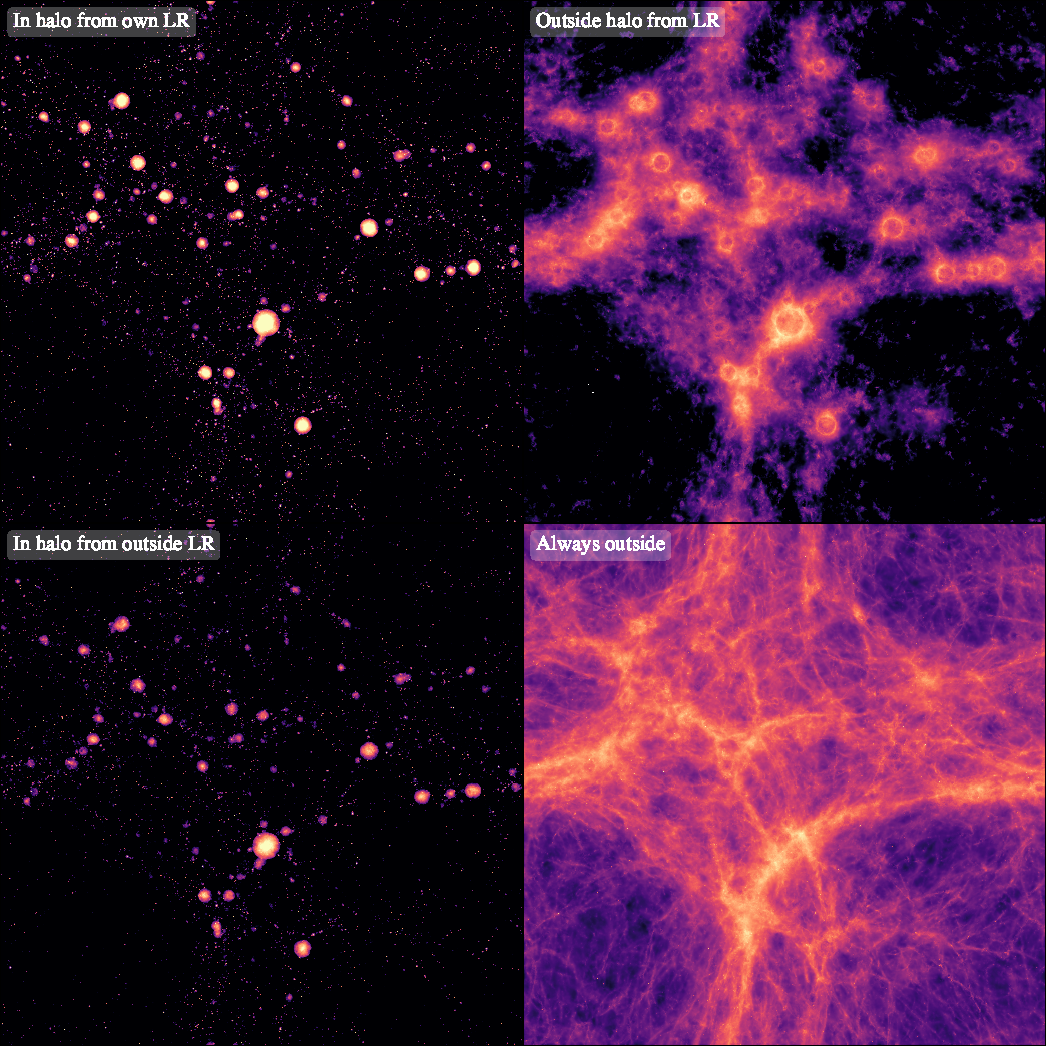
\includegraphics{figures/s50j7kAHF/four_images_magma_AHF.pdf}
    \caption{Gas distribution in the fiducial \simba{} model for the full
    $50\hmpc{}$ volume, split by the following Lagrangian components
    (clockwise, starting from top left): particles that began in Lagrangian
    regions at $z=99$ and have remained in the associated haloes at $z=0$;
    particles that began in Lagrangian regions and ended up outside of the
    destination halo; particles that began outside any Lagrangian region and
    ended up outside any halo; and particles that ended up in a halo but
    originated outside any Lagrangian region. All images are shown with the
    same (logarithmic) colour-map and normalisation and taking their linear
    sum would reproduce the full gas distribution at $z=0$. Gas particles
    that began in Lagrangian regions but ended up outside of haloes (top
    right) show a striking similarity to the distribution of gas with the
    33\% highest spread distance shown in Fig.~\ref{fig:bigdistanceimage}.
    As expected, particles that began outside of Lagrangian regions and
    remained outside of haloes (bottom right) trace the filaments and voids.}
    \vspace{1cm}
    \label{fig:lrtransfer}
\end{figure*}

\section{Lagrangian baryon transfer}
\label{sec:transfer}

We have explored the relative motion of dark matter and baryons using a
particle-level metric, showing that AGN jets in the \simba{} cosmological
simulations can spread baryons up to $12\hmpc{}$ relative to the neighbouring
dark matter. In this section, we consider the movement of baryons relative to
dark matter haloes and their corresponding Lagrangian regions. The definitions of
haloes and Lagrangian regions used here are described in \S \ref{sec:simba}.

This topic has been considered recently by \citet{Liao2017}, where they used
a $10\hmpc{}$ non-radiative simulation to show that the gas in haloes may
originate from different places than the dark matter in those same haloes in
the initial conditions.

\subsection{The different origins of baryons and dark matter in haloes}

Fig. \ref{fig:bigtransferpic} illustrates the mixed origins of the gas and
dark matter components in bound structures at $z=0$ by showing simultaneously
the initial and final states of the simulation. A common trend for all haloes
is a shell of gas around the main dark matter component in the initial
conditions, showing that gas in general is able to collapse further (due to
cooling and other processes) than the dark matter, which is unable to lose
angular momentum as efficiently. This is consistent with the larger values of
the spread metric for gas in haloes relative to the dark matter in haloes, as
shown in Fig. \ref{fig:distbaryon}.

The origin of the dark matter in the initial conditions corresponds exactly
to our definition of Lagrangian region for that component in \S
\ref{sec:simba}. These Lagrangian regions have very complex shapes, with
larger haloes tending to have more spherical Lagrangian regions, as can be
seen with the largest halo in the box (Group 0) in Fig.
\ref{fig:bigtransferpic}. These complex non-spherical shapes are why we
chose to identify our Lagrangian regions for gas through neighbour searching,
as other methods (e.g. constructing a convex hull enclosing all dark matter
particles that end up in a given halo) would not allow us to capture the
surprisingly intricate structure that is at play here.

There are many possible reasons for the complex shapes that we see here.
Consider a simple case where we have one `main' halo, and a satellite that is
being accreted. The gas and dark matter in the satellite galaxy have several
potential fates. For instance, when accreting onto the main halo, the gas in
the satellite may be shock heated, and stalled in the CGM, with the dark
matter being able to continue to move towards the center of the main halo.
This process dynamically separates the dark matter and gas, and now the gas
may have several fates; it could be pushed out in a feedback event, rise out
of the halo due to buoyancy, or fall to the centre of the halo after cooling
and re-join the dark matter. Once the gas has been removed from the CGM into
the IGM, it is free to be picked up by other passing galaxies.

The other possibility for the fate of this substructure is the dark matter
failing to accrete onto the central. In this case, the dark matter continues
moving out into the IGM, with the gas being shocked and captured by the main
halo. It is this complex difference in assembly between dark matter and
baryons, due to the latter behaving as a collisional fluid, that we aim to
capture here.

\subsection{Computing transfer between Lagrangian regions}

Given the definitions of haloes and Lagrangian regions in
\S \ref{sec:simba}, it is possible to classify every particle in the
simulation according to their Lagrangian ID and halo ID (if any) in the
initial and final conditions. The algorithm is as follows:

\begin{enumerate}
	\item ID match all particles between the initial and final conditions, including
	      star particles (these are matched to their gas progenitor). Black holes are ignored in this analysis since globally they represent a minimal amount of mass.

	\item Every particle at $z=0$ has several possible final states and origins, based on its halo ID ($i$) and Lagrangian region ID ($j$):
	      \begin{itemize}
	            \item Particle resides in  halo ($i \neq -1$)
	            \begin{itemize}
	           		\item Particle originated in the same Lagrangian region, $j = i$
	           		\item Particle originated outside any Lagrangian region, $j \equiv -1$
	           		\item Particle originated in some other Lagrangian region, $j \neq i$
	            \end{itemize}
	            \item Particle resides outside of any halo ($i \equiv -1$)
	            \begin{itemize}
	            	\item Particle originated outside any Lagrangian region, $j = i$
	            	\item Particle originated in some Lagrangian region, $j \neq i$
	            \end{itemize}
	      \end{itemize}
	      
	\item For every halo and Lagrangian region, the mass originating from each
	      of the above components is computed and stored.
\end{enumerate}



A visualisation of this particle classification scheme is shown in
Fig.~\ref{fig:lrtransfer}, where we split the gas distribution in the
\simba{} $50\hmpc{}$ box into the four main Lagrangian components that we
consider in the remainder of this paper. Considering each panel clockwise
from the top left, we select first the gas that is in the same halo at
redshift $z=0$ as the Lagrangian region that it originated in. As expected,
we see a population of spherical shapes corresponding to every halo in the
box, with their sizes corresponding to $R_{\rm vir}$ as defined by AHF. The
centers of haloes, where the gas is densest, are the brightest.


In the top right panel we have the gas that is outside any halo at $z=0$, but
is assigned to a Lagrangian region at $z=99$; this is the gas that should
have ended up in haloes by the end of the simulation if the baryonic matter
was also collisionless. We see that this component traces gas primarily
around massive haloes, resembling the large-scale bubbles that the AGN jets
power in \simba{} \citep{Dave2019}. Note that some of this gas piles up just
outside of haloes due to the somewhat arbitrary boundary defined by the
virial radius of haloes. This gas resides primarily in filaments, with some
reaching out into the voids.

In the bottom right panel, we visualise the gas that begun outside any
Lagrangian region and resides outside any halo at redshift $z=0$. This gas
traces the majority of the filamentary structure, and shows all of the
structure in the voids. 

Finally, in the bottom left panel, we have the gas that is in haloes at $z=0$
but originated from outside any Lagrangian region. As expected, this shows a
very similar structure (albeit less bright) to the gas that resides in its
own halo (top left), but this component originates from regions where the
dark matter now resides outside of haloes. This gas is likely dragged into
these bound structures by cooling flows, while the dark matter
is not able to lose angular momentum quickly enough to assemble by $z=0$.




\subsection{Transfer in a non-radiative Model}

\begin{figure}
	\centering
	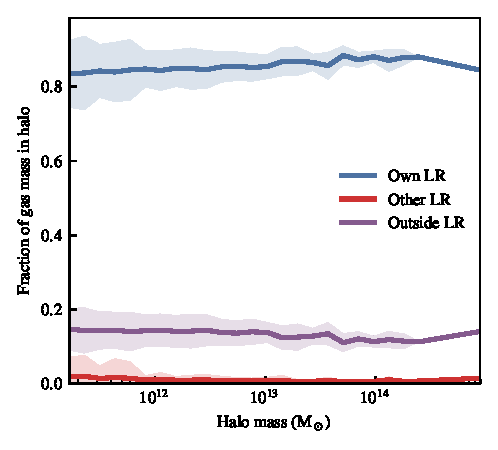
\includegraphics[width=\columnwidth]{figures/s50gadget/component_fraction_vs_halo_mass_gas.pdf}
	\vspace{-0.7cm}
 \caption{ The fraction of baryonic mass originating from each Lagrangian
 component in the non-radiative model (i.e. without sub-grid physics) is
 shown as a function of redshift $z=0$ halo mass. The gas particles are
 binned by their origin, with the baryons originating from their own
 Lagrangian region shown in blue, the Lagrangian region of other haloes
 (red), and outside of any Lagrangian region (purple). Shaded regions show
 the $1\sigma$ scatter in a given bin, which is given by one standard
 deviation of variation. The lines represent the mean value within each bin.
 Approximately 85\% of the baryonic mass of a given halo originates from its
 own Lagrangian region, showing very little transfer of baryons from either
 outside or from another Lagrangian region. This is provided for comparison
 to the full model result in Fig. \ref{fig:maintransferresult}.}
	\label{fig:nonradiativetransfer}
\end{figure}


Before considering the numerical results of the full model, we first present
the non-radiative simulation as a null model to investigate the effects of
hydrodynamics alone. In this case, we run the simulation without cooling,
star formation, or feedback, only including hydrodynamics, cosmology, and
gravity. In Fig. \ref{fig:nonradiativetransfer} we present the fraction of
baryonic mass for each halo contributed from each Lagrangian component, as a
function of halo mass. The blue line shows the fraction of mass in each halo
from its own Lagrangian region (top left in Fig. \ref{fig:lrtransfer}), the
red shows transfer into a halo from another Lagrangian region, and the purple
line shows the fraction of baryonic mass from outside any Lagrangian region
(bottom left in Fig. \ref{fig:lrtransfer}). There is no dependence on halo
mass (as the simulation is effectively scale-free above some resolution
limit), and apart from some small level of transfer from outside any
Lagrangian region (of around $10-15\%$), the baryonic mass in each halo
consists of that which originated in its own Lagrangian region.

The difference in origins of the baryons in the final haloes, from
hydrodynamical effects alone, is then around the $10-15\%$ level. This is
close to the 25\% level of segregation between gas and dark matter reported
by \citet{Liao2017} (who also used a non-radiative simulation), with the
difference likely rooted in the definitions that we use. We consider the
fraction of gas particles in the final redshift $z=0$ halo whose initially
pairing dark matter is also resident in that halo; hence what we are really
counting is the `contamination' of the halo by gas particles from outside of
its Lagrangian region. \citet{Liao2017} count all particles in the final
halo, treating gas and dark matter equally, then finding all particles that
were gas-dark matter pairs in the initial conditions. Their higher level of
segregation is expected due to contributions from dark matter particles that
are resident in a halo but whose initial gas pair is not. Fundamentally this
represents the difference in our approaches; here we are interested in
treating the dark matter as a ground source of truth, and asking if the gas
nearest to that dark matter follows it into the same haloes.
\citet{Liao2017}, on the other hand, were interested in treating \emph{all}
occupants of the final halo as the ground source of truth, and asking what
differences there were in their origin.

The causes for our contamination here are less clear than in the case of
\citet{Liao2017}; we would report a halo that has had gas only \emph{removed}
as being completely uncontaminated, and hence stripping of gas is
an unsatisfactory explanation of these differences. The likeliest explanation
for the contamination in this case is that the baryons and dark matter go through
a phase of mixing as they enter the cosmic web, before going on to fully
collapse into bound structures.


\subsection{Transfer \emph{into} haloes}
\label{sec:transferinto}


\begin{figure*}
	\centering
	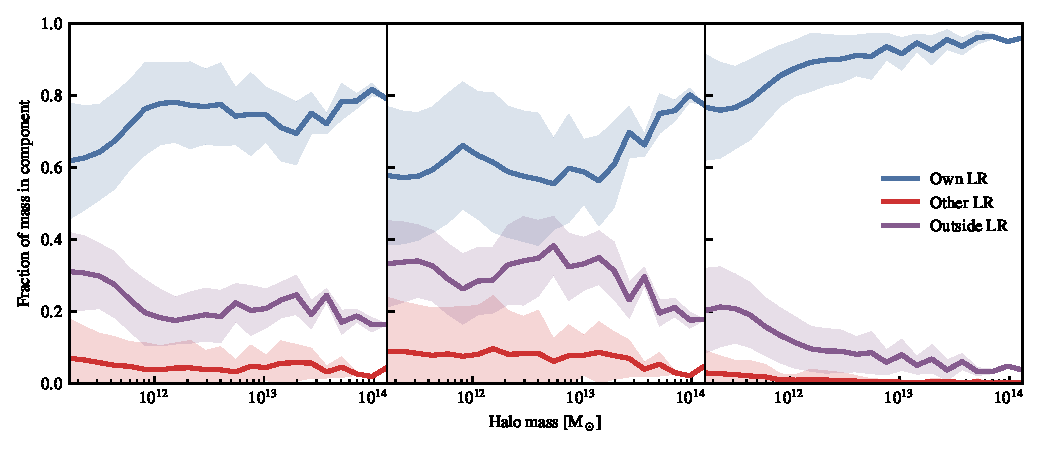
\includegraphics{figures/s50j7kAHF/component_fraction_mixed.pdf}
	\vspace{-0.7cm}
	\caption{
  The fraction of baryonic mass in haloes at $z=0$ originating from their own
  Lagrangian region (blue), the Lagrangian region of other haloes (red), and
  outside of any Lagrangian region (purple), shown as a function of $z=0$
  halo mass for the fiducial \simba{} model. We consider all baryons in
  haloes (left) as well as their gas (center) and stellar (right) components
  separately.
	}
	\label{fig:maintransferresult}
\end{figure*}

Moving on to the full \simba{} model, we consider again the fractions of
baryonic mass as a function of halo mass, split by Lagrangian component. Fig.
\ref{fig:maintransferresult} shows three panels: the left panel shows all
baryons, the centre shows only gas, and the right panel shows the
contribution from only the stars. The lines are coloured the same as the
non-radiative model shown in Fig. \ref{fig:nonradiativetransfer}. Now that we
have introduced scale into the simulation through density-dependent energy
injection mechanisms, these components scale with halo mass. The general
trend is that for an increasing halo mass, a Lagrangian region is able to
hold on to more of the original baryonic mass, with this flattening off
around $M_H = 10^{12} \msolar$. For a given halo, significantly more of the
gaseous mass originates outside the original Lagrangian region as compared to
the stellar mass ($\sim 40 \%$ versus $\sim 10 \%$). The transfer between
haloes is at around the $\sim 10\%$ baryonic mass level, with this transfer
predominantly originating from the gaseous component, as compared to the
stellar component. This combines nicely with the distance metrics shown in \S
\ref{sec:feedbackmetrics}, which showed that the dark matter and stars have
very similar dynamics and hence should be similarly well bound.


This transfer into, and between, Lagrangian regions can have several physical
origins. The first, as shown in the non-radiative run, is caused by the
collisional dynamics of the gas preventing gas from following the dark matter
in all cases. We found that this can account for up to 15\% of the baryonic
mass of a bound structure at redshift $z=0$ originating from a different
region than the dark matter (see Fig. \ref{fig:nonradiativetransfer}), but this
could not account for any \emph{inter-Lagrangian} region transfer.

The galaxy formation sub-grid model clearly has a significant effect on the
baryonic make-up of haloes at redshift $z=0$. The fraction of mass from
outside any Lagrangian region has increased to 20-40\%. This increase is
explained by the inclusion of sub-grid cooling and feedback processes, with
the baryons now able to cool before accreting and lose angular momentum at a
much higher rate than the dark matter component is able to.

Around 10\% of the baryonic mass of haloes is now made up of gas that has
experienced inter-Lagrangian transfer. It is important to recall that this is transfer
between bound structures at redshift $z=0$, and that it only takes into account
the initial and final conditions of the simulation; this analysis does not
consider the complete history of these particles.

The transfer between haloes has several possible sources: stripped gas from
nearby galaxies that are still classified as their own bound structures at
redshift $z=0$, gas that has been expelled from galaxies through stellar
winds or AGN feedback and re-captured by a halo, and transfer due to boundary
effects caused by the complex shapes of Lagrangian regions according to the
definition adopted. With the non-radiative simulation showing zero transfer
between haloes, and there being little transfer before $z=2$ in the fiducial
model (see below in Fig. \ref{fig:ltzevo}), we believe that the contribution
from pure dynamics alone to inter-Lagrangian transfer is likely very small.
When repeating this analysis with the \nojet{} run, the inter-Lagrangian
transfer is reduced, but still remains at the 10\% level. The feedback events
that power this transfer must be dominated by the expulsion (or alternatively
preventative pathways) from stellar winds and the residual thermal AGN
feedback.

A given mass bin contains haloes that entertain a range of 10x in transfer,
which is likely dependent on environment. Future work should investigate in more detail
the physical mechanisms driving the scatter in these relations.

The level of transfer above a halo mass of $10^{13} \msolar{}$ must be
interpreted carefully, as there are very few haloes above this mass present
in the box (less than 50), with the small scatter being misleading. It is
also important to note that the shaded regions in Fig.
\ref{fig:maintransferresult} represent the $1\sigma$ scatter in a given bin
and explicitly do \emph{not} include any dispersion that would occur from a
finite sampling of haloes or halo assembly bias.

\subsection{Redshift evolution of transfer into haloes}

\begin{figure}
    \centering
    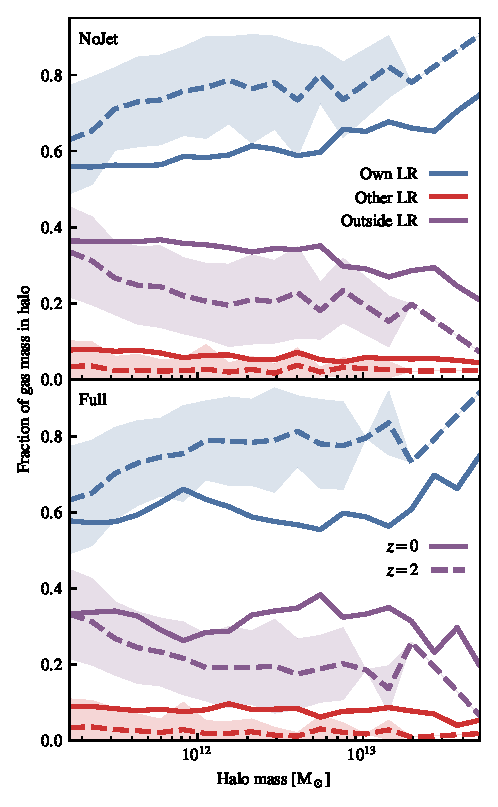
\includegraphics[width=\columnwidth]{figures/component_fraction_multi_z.pdf}
    \vspace{-0.7cm}
    \caption{The fraction of gas mass in haloes at redshift $z=0$ (solid) and
    redshift $z=2$ (dashed) as a function of halo mass at that redshift, split by
    Lagrangian component. Scatter is shown only for the $z=2$ results. The top panel
    shows the results from the \nojet{} simulation, with the bottom showing the
    full \simba{} model.}
    \label{fig:ltzevo}
\end{figure}

To further investigate the origin of the inter-Lagrangian transfer, in Fig.
\ref{fig:ltzevo}, we consider the \nojet{} model and show how the gas in
haloes at redshift $z=2$ is composed in this and the full \simba{} model.

We see that both the \nojet{} and \simba{} models broadly reproduce the same
fractions of gas in each Lagrangian component, with some interesting differences.
In the full model, a higher fraction ($25-50\%$) of the halo gas originates
from inter-Lagrangian transfer than the \nojet{} model at all masses, with no
change in the shape of this function observed. The fraction of gas
originating outside of any Lagrangian regions shows a dip at around
$10^{12}\msolar{}$ being removed in the \nojet{} model, however this is well
within the scatter that we observe in the full model results.

All of this is despite both models producing very different $z=0$ halo baryon
fractions (see Fig. \ref{fig:baryonfraction} for the full model; the \nojet{}
model produces baryon fractions at approximately the cosmic mean for all halo
masses above $\sim10^{11}\msolar{}$). For a further investigation, halo matching
should be performed between the two models and individual cases compared, but
this is out of the scope of the current work.

The fraction of gas in haloes originating from the different Lagrangian
components shows a closer match at $z=2$, with the shape and
normalisation of all components being well within the reported scatter. The
higher-mass end of these results ($M_H > 10^{13}\msolar{}$) also lacks
objects here, with there being even fewer in this mass range than at $z=0$.

We see that between redshift $z=2$ and $z=0$ a change in the slope
of these functions takes place, and that the level of inter-Lagrangian transfer
increases significantly. The fraction of gas originating from the Lagrangian 
regions of other haloes increases by a factor of two (or more) at all halo
masses, with the fraction of transfer from outside Lagrangian regions remaining
constant or again increasing by a factor of two dependent on the resident halo mass.

All of this must be explained within the context of very different baryon
fractions for all haloes at $z=0$. One possibility is that the majority of
gas gained from outside of a haloes own Lagrangian region remains in the CGM,
with very little of it making it into the disk (this is supported by the very
low fraction of halo stars that originate from transfer, see Fig.
\ref{fig:maintransferresult}). This gas can then be swept out of the halo
either by stellar winds or (ejective) AGN feedback. Alternatively, if the
main pathway for feedback is preventative, and the gas outside of haloes is
well mixed, then this assembly of baryons would be curtailed equally for all
Lagrangian components. A further investigation of these transfer properties
(considering differences between the galaxy disks and the CGM) would be well
suited for follow-up work using higher resolution simulations.

\subsection{Transfer \emph{out} of Lagrangian Regions}

\begin{figure}
	\centering
	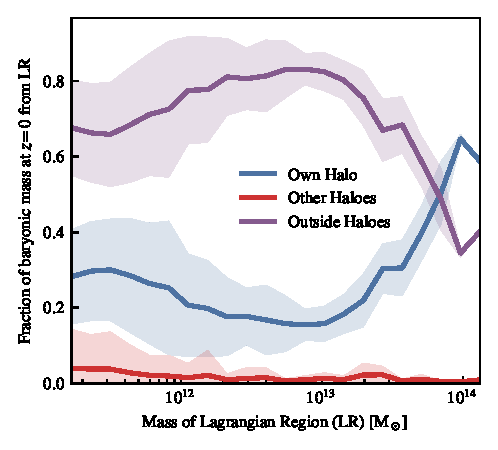
\includegraphics{figures/s50j7kAHF/inverse_component_fraction.pdf}
	\vspace{-0.7cm}
 \caption{The fate of gas that begins in Lagrangian regions, as a function of
 initial Lagrangian region mass. The blue line shows the fraction of baryons
 that reside in the halo that defines the Lagrangian region at redshift
 $z=0$, the red line shows the the fraction of baryons that lie in a
 different halo, and the purple line shows the baryons that lie outside of
 any halo at redshift $z=0$. All but the most massive objects in the box
 struggle to retain more than 30\% of their baryons due to various factors,
 see the text for details. The fraction of mass retained in the corresponding
 halo (blue) is the lowest in the mass range $10^{12} - 10^{13}\msolar{}$.}

	\label{fig:transferoutoflrs}
\end{figure}



Let us now consider the fates of baryons that begin their lives in Lagrangian
regions. This material has three possible fates, as shown in Fig.
\ref{fig:transferoutoflrs}: it can end up in the same halo as the dark matter
from that Lagrangian region (blue line), in another halo (red line), or
outside of any halo in the IGM (purple line). Here, we we plot the fraction
of LR mass at $z=0$ from each component as a function of their Lagrangian
region mass (this is the sum of the baryons and dark matter contained within
that Lagrangian region). The Lagrangian region mass is somewhat higher than
the eventual halo mass due to the baryon fractions of redshift $z=0$ haloes
being below the cosmic mean. We see that, below a halo mass of
$10^{13.5}\msolar{}$, only around 20-30\% of the baryons initially present in
the Lagrangian region make it in to the halo by $z=0$. Only above a halo mass
of $10^{13.5}\msolar{}$ do haloes become strong enough attractors to retain
the majority of their baryons. Despite the clear trend, this result is
somewhat uncertain due to the very small number of these very large haloes
present in our $50\hmpc{}$ box. On top of this initial structure, we see that
there is a dip in the retained fraction of baryons between $10^{12}$ and
$10^{13}\msolar{}$. We speculate that this is due to the increased efficiency
of AGN feedback in haloes in this mass range, allowing for more gas in
central objects to be expelled, however making a direct connection would
require significant investigation. It is worth noting that without the AGN
jets (i.e. in the \nojet{} run), the baryon fraction of haloes in this mass
range is approximately $f_b / f_{b,c} = 1$.

Finally, we find that up to 10\% of the Lagrangian region gas of low-mass
haloes ($<10^{12} \msolar{}$) can be transferred to other haloes, decreasing at
higher masses. A larger cosmological volume with more objects is required for
a full study of objects at masses higher than $M_H > 10^{13}\msolar{}$, but
these trends point towards inter-Lagrangian transfer being fuelled by
accretion of gas that is either expelled or stripped from lower mass haloes
by higher mass objects. A plausible physical scenario is that early
feedback leading up to redshift $z=2$, where star formation (and hence
stellar feedback) peaks, expels significant quantities of gas from lower mass
haloes that can then be swept up at later times from the IGM by all haloes.
Higher mass haloes at this redshift may have a strong enough gravitational
potential to enable their stellar winds to be more efficiently recycled,
preventing them from being sources of inter-Lagrangian transfer.

The combination of the baryons that are retained by haloes (Fig.
\ref{fig:transferoutoflrs}) and the baryons that they manage to accrete from
sources outside their Lagrangian region (Fig. \ref{fig:maintransferresult})
is seen in the baryon fraction of haloes, shown in Fig.
\ref{fig:baryonfraction} split by Lagrangian component. Here, we split the
overall baryon fraction (relative to the cosmic mean) into three Lagrangian
components, coloured by the baryons from the haloes own Lagrangian region
(blue), other Lagrangian regions (red), and from outside any Lagrangian
region (purple). In general, we see that there is a trough in the baryon
fractions of haloes with a mass between $10^{12}\msolar{}$ and
$10^{13}\msolar{}$, with the baryon fraction reaching the cosmic mean for the
largest objects in the box (with a halo mass of $10^{14}\msolar{}$). The
baryon fraction returning to $f_b = 1$ for these very large haloes is not due
to these haloes retaining all of their Lagrangian gas, however; it is a
complex interplay between their accretion from outside, from other Lagrangian
regions, and from the significant component that originates outside of any
Lagrangian region. These objects are clearly able to mix outside of their
halo boundaries, swapping gas with the IGM, as has been shown in several
studies through `splashback' \citep{Mansfield2017, Diemer2017}.

The dip in baryon fraction between $10^{12}\msolar{}$ and $10^{13}\msolar{}$ in halo
mass corresponds to the dip in retained baryons in a similar mass range in
Fig. \ref{fig:transferoutoflrs}. However, within this mass range, it appears
that the fraction of baryons originating from outside the Lagrangian region is
more significantly affected than the fraction of baryons from the haloes own
Lagrangian region (reduced by 50\% as opposed to 20\%). This points
to a more complex accretion history for these objects, with a mixture of
ejective feedback (in general reducing the amount of retained baryons) and preventative
feedback (in general reducing the amount of baryons from outside of the
corresponding Lagrangian region) shaping their baryonic content.


\begin{figure}
	\centering
	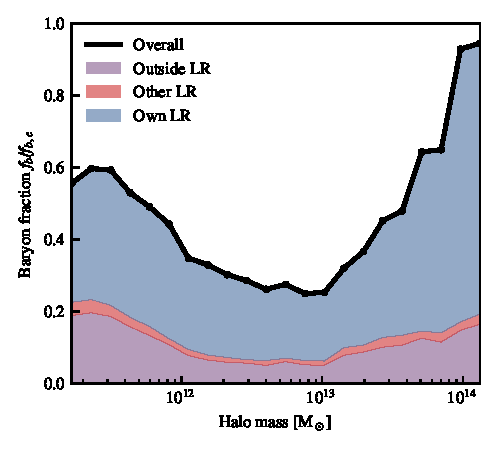
\includegraphics{figures/s50j7kAHF/baryon_fraction_breakdown.pdf}
	\vspace{-0.7cm}
	\caption{The baryon fraction $f_b$ relative to the cosmic baryon fraction
	$f_{b, c}$ shown as a function of halo mass. The coloured bands show the
	contributions to the baryon fraction from various Lagrangian components.}
	\label{fig:baryonfraction}
\end{figure}